
\documentclass[10pt, conference, compsocconf,a4paper]{IEEEtran}

\usepackage[pdftex]{graphicx}

% correct bad hyphenation here
\hyphenation{op-tical net-works semi-conduc-tor}


\begin{document}
\title{Extending Mocapy++ with a mixed probability distribution\\Advanced Topics In Data Modeling}

\author{\IEEEauthorblockN{Kasper Nybo Hansen}
\IEEEauthorblockA{Dept. of Computer Science\\
University of Copenhagen\\
Copenhagen, Denmark\\
nybo@diku.dk}
}

% make the title area
\maketitle

\begin{abstract}
Mocapy++ is a C++ toolkit for learning and inference in dynamic Bayesian networks. This report describes the implementation, testing and results of extending Mocapy++ with a new node. 

The new node is a mixed node, allowing both discrete and continuous values. The continuous part of the node is a gaussian distribution. The new node is used to calculate a probabilistic model of hydrogen bonding in protein structures. The probabilistic model is learned from a provided dataset.
\end{abstract}

\begin{IEEEkeywords}
Mocapy++; DIKU; Dynamic Bayesian networks; Mixed probability distribution
\end{IEEEkeywords}


\section{Introduction} % (fold)
\label{sec:introduction}

% http://www.stat.uiowa.edu/~nshyamal/22S175/DI.pdf
% 
% http://www.tutorvista.com/math/mixed-probability-distribution
% http://www.freemathhelp.com/forum/viewtopic.php?f=12&t=34692
% 
% Good explanation
% http://www.ds.unifi.it/VL/VL_EN/dist/dist3.html

An introduction with a short discussion of the theory of inference and learning in Bayesian networks, relevant to Mocapy++.


\subsection{Dynamic Bayesian Network} % (fold)
\label{sub:dynamic_bayesian_network}
A Bayesian network consists of a Directed Acyclic Graph where the nodes are random variables. Each edge in a Bayesian network represents a probabilistic dependency. More precisely figure \ref{fig2} shows a Bayesian network where the probability of observing $o1$ is dependent on $h1$. We call the node $o1$ the observed node and $h1$ and $h2$ the hidden nodes. 

\begin{figure}[ht]
\centering
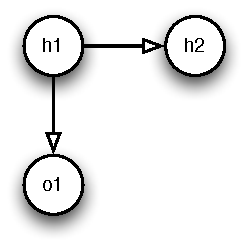
\includegraphics[width=0.1\textwidth]{figures/fig2.pdf}
\caption{Example of the bayesian network}
\label{label}
\end{figure}
% subsection dynamic_bayesian_network (end)

\subsection{Mixed node} % (fold)
\label{sub:mixed_node}
The implemented mixed node takes exactly one discrete parent. The parent node can have any size $n$, i.e. it can take on integer values in the range $[0,n]$.
% subsection mixed_node (end)


\subsection{Mixed distribution} % (fold)
\label{sub:mixed_distribution}
The mixed distribution can be divided into two parts. A discrete and continuous part. Let $X$ be a random variable that takes values in the set $S$. We then define the discrete part as the countable set $D \subseteq S$, and the continuous part as $C \subseteq S$. We define a mixed distribution as a distribution that has the following two probabilities

\begin{itemize}
  \item $0 < P(x \in D) < 1$
  \item $P(x \in C) = 0$
\end{itemize} 

The discrete part of the distribution can be described by a distribution table. The table will in the implemented node consist of two entries, that sums to exactly $1$. The first entry describes the probability of the node being a discrete node, the second entry describing the probability of the node being a continuous node. Define $P(X = discrete)$ as the probability that the node is discrete, and $1-P(X = discrete)$ as the probability that the node is continuous. 

The continuous part of the mixed distribution consist of the Gaussian distribution aka. the normal distribution. The Gaussian is defined as

\begin{equation}
f(x;\mu,\sigma) = \frac{1}{\sqrt{2\pi\sigma^2}} e^{ -\frac{(x-\mu)^2}{2\sigma^2} }  
\end{equation}
where $\mu$ is the mean value, and $\sigma$ is the standard deviation.

We wish to estimate the parameters of the discrete and continuous distribution. We can do this by the maximum likelihood method. For the discrete case, the maximum likelihood can be calculated as

\begin{equation}
  \hat{P}(X = discrete) = \frac{\#discrete}{\#total} 
\end{equation}
and
\begin{equation}
  \hat{P}(X = continuous) = 1 - \hat{P}(X = discrete)
\end{equation}

when estimating the Gaussian variables $\mu$ and $\sigma$ we use the maximum likelihood function for the Gaussian, i.e.
\begin{equation}
  \ln(\mu, \sigma^2) = -\frac{n}{2}\ln(2\pi) - \frac{n}{2}\ln\sigma^2 - \frac{1}{2\sigma^2}\sum_{i=1}^n (x_i-\mu)^2.
\end{equation}
we wish to maximize this function, so we take the derivative and find the stationary points. Doing this yields
\begin{equation}
  \hat{\mu} = \overline{x} \equiv \frac{1}{n}\sum_{i=1}^n x_i, \qquad \hat{\sigma}^2 = \frac{1}{n} \sum_{i=1}^n (x_i - \overline{x})^2
\end{equation}


% subsection mixed_distribution (end)

% subsection d (end)

\subsection{Applications to Hydrogen bounding} % (fold)
\label{sub:applications_to_hydrogen_bounding}
The mixed distribution applies to hydrogen bonding in the following way. A hydrogen bound has two states:

\begin{itemize}
  \item A bond does not exist
  \item A bond exists with a energy $E$
\end{itemize}

Under the assumption that the energy of a hydrogen bonding can be modeled by a Gaussian probability distribution we can model a hydrogen bond in the following way. The discrete distribution is modeling the first boolean case, i.e. "Is the bond present or not?". If the bond is present, the Continuous part can be used to to find the energy, $E$, of the bond.


% subsection applications_to_hydrogen_bounding (end)


% section introduction (end)

\section{Implementation} % (fold)
\label{sec:implementation}

\subsection{Adding the mixed node} % (fold)
\label{sub:adding_the_mixed_node}

% subsection adding_the_mixed_node (end)

There are two main steps in the framework. The first step is the \emph{E-step}. The E-step is the inference step, where the values of the hidden nodes are inferred by using the set of samples generated by the sampler. The sampler used in this project is the Gibbs sampler that comes with Mocapy++.

Each time a node is sampled the \textbf{E}xpected \textbf{S}ufficient \textbf{S}tatistics (ESS) class is updated. The ESS class acts as a container where the data neccessary to calculate the nodes parameters are stored. For the mixed node, this means storing the following data:

\begin{itemize}
  \item Number of discrete and continuous observations
  \item The energy stored in a way so the Gaussian model parameters can be calculated
\end{itemize}
the parameters needs to be stored for each value that the parent node can take. I.e the size of the tables stored in the ESS, depends on the size of the parent node.

A description of the implementation of the mixed distribution in Mocapy++. 

A mixed node has the following parameters, CPD, mean and variance. The CPD determines the relationship between the continuous and discrete distribution. It is a table of probabilities, where.

The mean and variance is parameters used in the continuous part of the distribution, more precisely in the Gaussian distribution. 
                                                                                                                                  

When instantiating a new node, it is possible to ask the node to take on random values. Furthermore it is possible to specify the CPD, mean and variance. If nothing is specified the node is initialized with a uniformly distributed CDP, and random values for the mean and variance. 

In this report we assume that the node size of our mixed node is always $2$, this assumption also has the effect that the Gaussian is in 1d. If the mixed node should be expanded to handle multidimensional gaussian, the node size should be variable.


\subsection{ESS} % (fold)
\label{sub:ess}
I have implemented the ESS class in the file \texttt{mixed/mixedess.cpp}. The class is responsible for collection data about the sample points, so they can be used later in the density class. Both tables are stored in the ESS array.

The mixedess class stores two tables for later retrieval in the density class. 

Both tables are populated in the class method \texttt{add\_ptv}. This method takes a vector as input. The vector has the format
\begin{equation}
  \{Parent\ value, Indicator, Energy\}
\end{equation}

If $Indicator=0$ then we know that the sample is a discrete sample, otherwise it must be a continuous sample.

The first table stores the number of observations of discrete and continuous nodes. It has size equal to the parent size $\times$ node size. The table has a row for each value the parent can take. For each value of the parent the ESS thus stores the number of discrete and the number of continuous nodes. Define the parent with value $i$ as $p_i$, and define the size of the parent node as $n$. Then the following table yields an outline of the first table stored in the ESS
\begin{center}
  \begin{tabular}{c | c | c}
  $p_0$ & \#Discrete obs for $p_0$ & \#Continuous obs for $p_0$ \\
  $p_1$ & \#Discrete obs for $p_1$ & \#Continuous obs for $p_1$ \\
  \vdots & \vdots & \vdots \\
  $p_{n-1}$ & \#Discrete obs for $p_{n-1}$ & \#Continuous obs for $p_{n-1}$ 
  \end{tabular}  
\end{center}
where \# means `number of' and obs is a abbreviation for observations.

The second table stored in the ESS has the size parent size $\times$ node size. For each parent value we store two entities. The first entity is the sum of the energies, and the second is the sum of the squared energies. Define all the energy samples belonging to parent $p_i$ as $E_i$, then for each continuous sample with parent value $p_i$ we sum the energy in one column and the sum the energy squared in the other column. An outline of the table can be seen in the following table
\begin{center}
  \begin{tabular}{c | c | c}
  $p_0$ & $\sum_{\forall e \in E_0} e$ & $\sum_{\forall e \in E_0} e^2$ \\
  $p_0$ & $\sum_{\forall e \in E_1} e$ & $\sum_{\forall e \in E_1} e^2$ \\
  \vdots & \vdots & \vdots \\
  $p_{n-1}$ & $\sum_{\forall e \in E_{n-1}} e$ & $\sum_{\forall e \in E_{n-1}} e^2$ \\
  \end{tabular}  
\end{center}


%subsection ess (end)

\subsection{Densities} % (fold)
\label{sub:densities}
CPD = 2*parent size, each parent can yield a value, the indicator shows if it is continuous or discrete

The sampling returns a tuple where the first value is the indicator, and the second is the energy.

Problem with x=0

% subsection densities (end)
%section implementation (end)

\section{Testing of implementation} % (fold)
\label{sec:testing_of_implementation}

A description of some simple tests that show that the implementation is correct. 

\subsection{Test of inference} % (fold)
\label{sub:test_of_inference}

% subsection test_of_inference (end)

\subsection{Test of sampling} % (fold)
\label{sub:test_of_sampling}
In this test I would like to confirm that the samples drawn from the mixed node corresponds to the nodes parameters.

In \texttt{examples/hmm\_mixed2.cpp} I have made a test of the sampling part of the mixed node. I have made the test by creating a DBN with randomly picked CPD, mean and variance. I have then sampled from this network yielding data points I can use to train a second network.

The 

In order to test the sample function, I have exported the sampled data points and made two histograms. The first histogram illustrates the discrete distribution, i.e. the contents of the CPD. This normalized histogram should resemble the randomly picked CPD.

The histogram should approximate a bell curve with mean and variance corresponding what is randomly generated. The histogram can be seen on figure \ref{fig1}. On top of the histogram, is plotted a Gaussian probability density function with the mean and variance equal to the randomly generated. As can be seen from the figure \ref{fig1} the histogram approxmiates the Gaussian well, and the conclusion must be that the samples drawn from the continuous part of the distribution is correct.

\begin{figure}
\centering
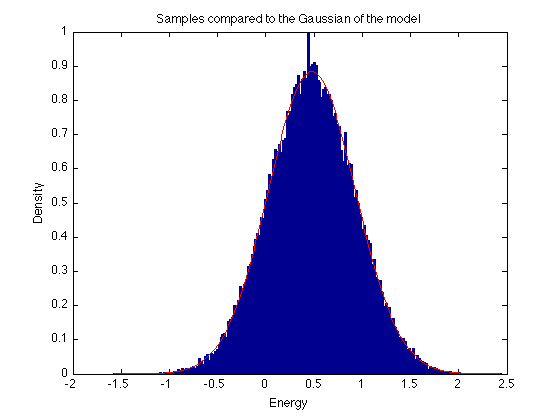
\includegraphics[width=0.5\textwidth]{figures/fig1.png}
\caption{Illustration of the samples drawn from the Gaussian part of the mixed distribution}
\label{fig1}
\end{figure}

%subsection test_of_sampling (end)

% section testing_of_implementation (end)

\section{Future work} % (fold)
\label{sec:future_work}
The present implementation does not enable the user to specify which distributions should be part of the mixed node. Future work could involve making use of the existing distributions and using them in the mixed node. This would remove the duplicate code that is present in the current prototype of the mixed node, and make the mixed node more flexible.
% section future_work (end)


\section{Results} % (fold)
\label{sec:results}

% section results (end)   



\bibliographystyle{abbrv}
\bibliography{bibliography}
\end{document}